\section{Finding \& Trends}
As we know, in \verb|OBS|, all intelligence resides in the edge nodes, which are at the same time the buffer and the processor on the network.     Simply put, current congestion control scheme are same pattern. They all gathering network state information first. Setup a certain threshold to estimate the congestion state. And then send a customize message to edge router according to the current network state. 


\begin{figure}[!htb]
    \label{fig:pattern}
    \begin{center}
        \leavevmode
        \ifpdf
        \resizebox{120mm}{!}{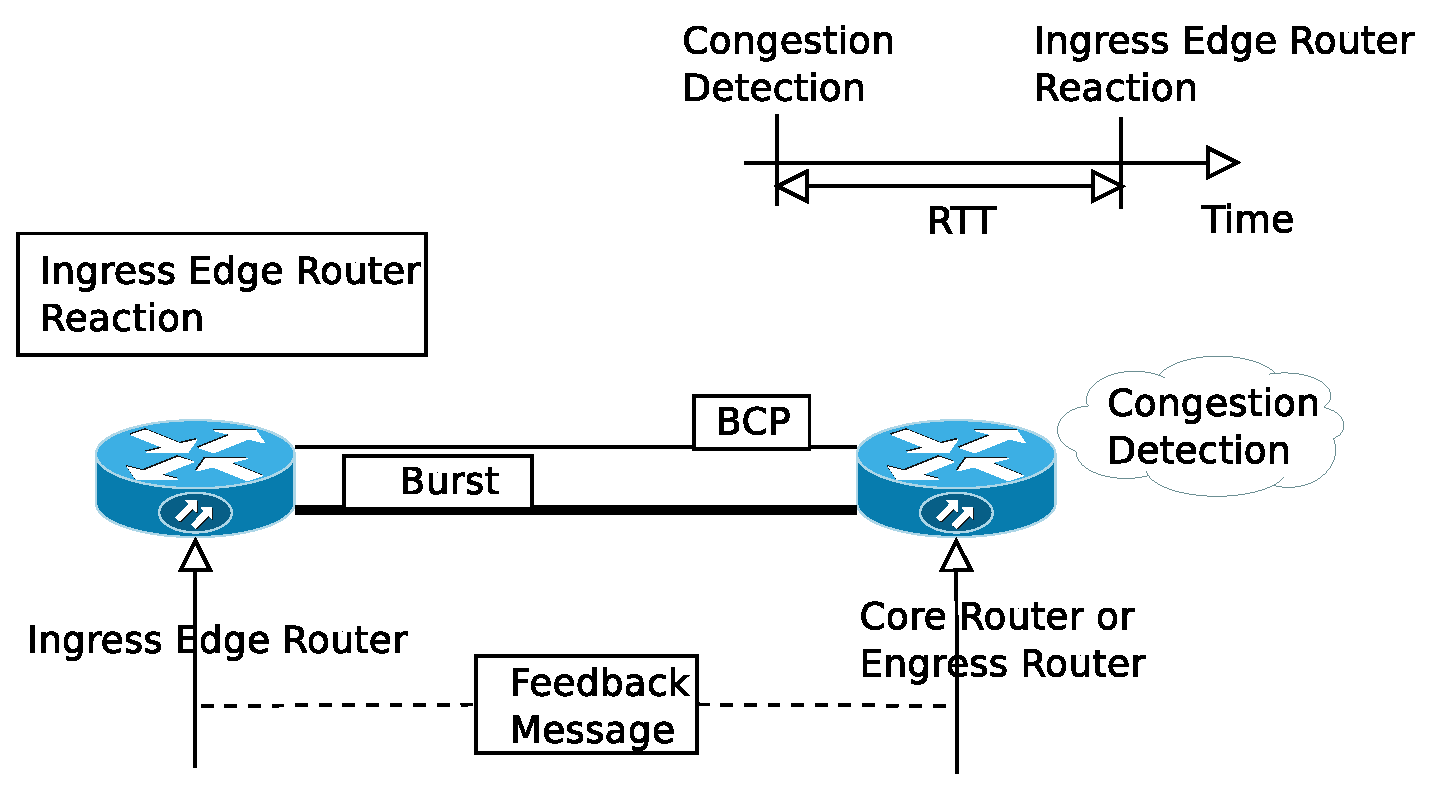
\includegraphics[height=6in]{pattern}}
        \else
        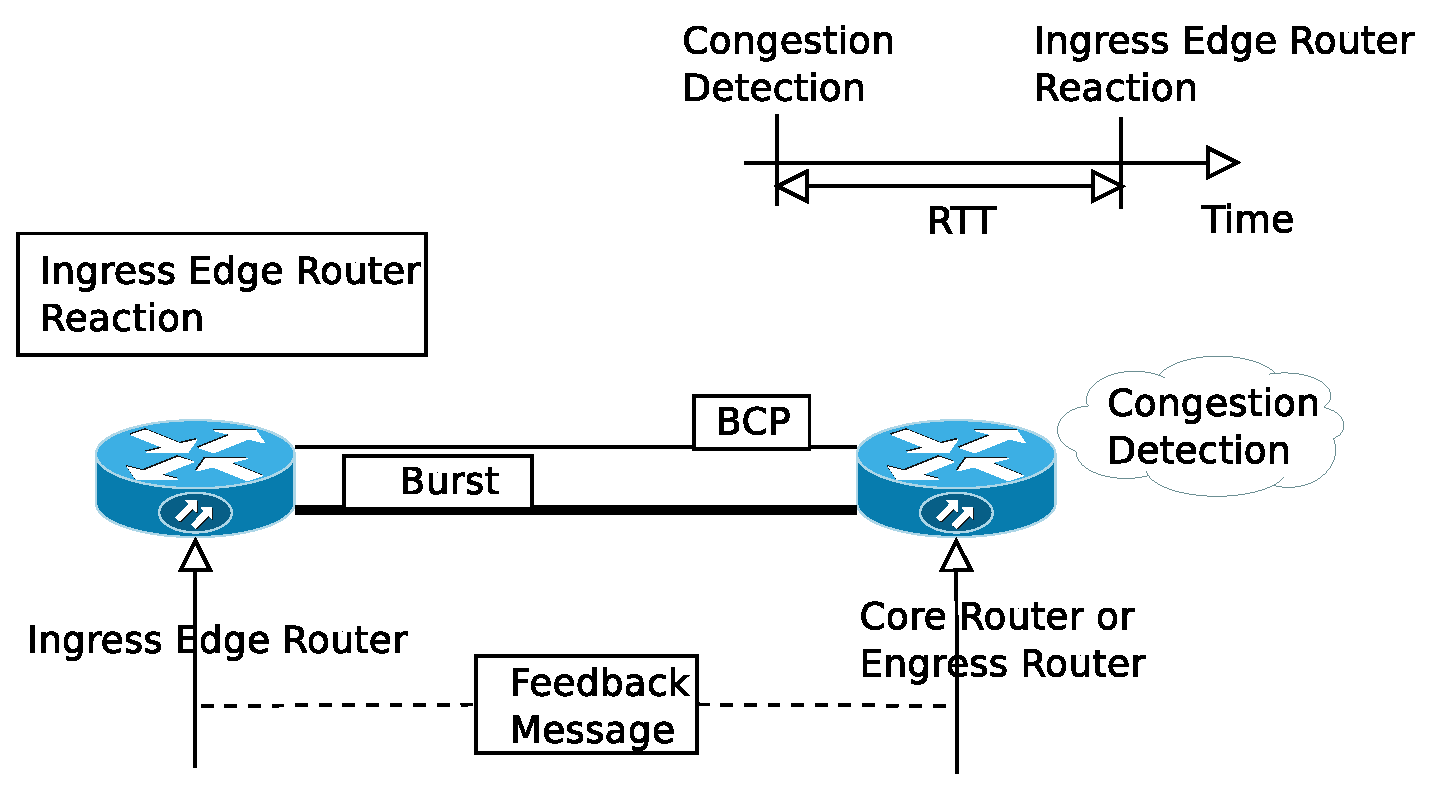
\includegraphics[bb = 92 86 545 742, height=6in]{pattern}
        \fi
        \caption{Pattern to control OBS congestion}
    \end{center}
\end{figure}

Figure \ref{fig:pattern} not only tell us the current popular pattern on research about OBS congestion control. It also tell us the steps to control congestion. This patter is practical and correct. So it will also be used in this study. Although the petter of vary congestion control mechanism are same. But there are a large amount difference among vary scheme in implementation detail. Such as different frequently to send feedback message to edge router, different way to
determine the congestion state threshold, different feedback message body. Certainly, they result in different performance. 

In their paper, they don't tell how to setup the threshold. They just give a final result. The value maybe have test a lot of times and they think that is proper for their model. It also is a constant value. But I think this value should adjust with the change of network topology. Besides, They don't tell how long is the RTT. The \verb|RTT| can use to measure the speed of ingress react. The \verb|Threshold| is a most important factor to affect the scheme to indicate congestion state or not.
But there is not a formula to got these two value through pure analysis. Current scheme just by trial and error to find a proper value for their simulation model.  

Moreover, Once their model is determined. All parameter is definite during simulation time. Include the most important \verb|Threshold| value. In my opinion, Congestion control is a dynamic optimization problem. This \verb|Threshold| should self-adjust accordingly. Burak Kantarci and Sema Oktug propose a congestion control scheme base on adaptive threshold \cite{adaptive}. The improvement is also very good. 

The previous researcher use throughput and loss ratio to measure their result. The higher throughput and the lower loss ratio. That will be propose as a better congestion control scheme. There also very important factor should be consider to determine whether a new scheme is better. That is whether as effective at high load as at low load. All previous researcher have pay much attention to this point. 

Previous mostly assume the burst arrive process follow the Poisson process and their lengths are negative exponentially distributed. But base on the some newest study. It has been shown that  whereas flow arrivals are Possion (or close to Possion), flow sizes are not exponential, but rather heavy-tailed, and thus they are closer to a Pareto distribution than an exponential one.  
